\section{Platform and applications}\label{sec:platform}

\evfut{} The platform described here does not exist. The PoC is one walking skeleton toward it, and a
gap candidate remains a prediction until a human answers it.

\paragraph{Three evidence worlds.} Every piece of evidence belongs to one world, already a typed field
in the code. \emph{World~A}, public evidence (textbooks, papers, standards, forums, public learner
data), can yield concepts and taught heuristics, but not episode-specific cues or local practice.
\evobs{} It is implemented for open-web text only. \emph{World~B}, organization-specific evidence
(procedures, tickets, commits, reviews, logs, incident reports), adds a second axis, practice:
prescribed (\code{imagined}), recorded (\code{done}) or reported. \evhyp{} The gap between imagined and
done is the organizational form of the residual. \evobs{} The schema exists; no ingestion does.
\emph{World~C}, human evidence (elicitation, ratings, learner responses, coder labels), has types but no
data. \evfut{} A and B build the reconstruction; the gap map predicts where C is needed; C answers through
the channel matched to the predicted knowledge type and is the only path that can score the predictions.
C never edits the reconstruction in place, and at least one human arm stays blind to the reconstruction,
or anchoring shrinks the measured residual.

\paragraph{Rules the platform keeps.} \evobs{} Labels are computed, never set. A label is only as strong
as its weakest link. Derived outputs (gap records, scores, questions) are \code{inferred} at best, and the
evidential gate refuses them as a criterion. \evfut{} Labels move up only through World~C or
cross-family verification; World~B claims never leave their organization's tenant; and
\textbf{unvalidated candidates never reach a learner or an end user}. No code enforces these three yet.
On premises, the platform needs three model families available locally (generator, verifier, closure
judge). \evobs{} The PoC already runs its judge locally, which shows the pattern is viable and also its
risk: that 7B judge did not beat its fair control. Organizational deployment adds per-user access control
propagated to claims, retrieved text treated as data and never as instructions, and a hash-chained audit
trail (Extended Technical Report, Section~18).

\begin{figure}[tbp]
  \centering
  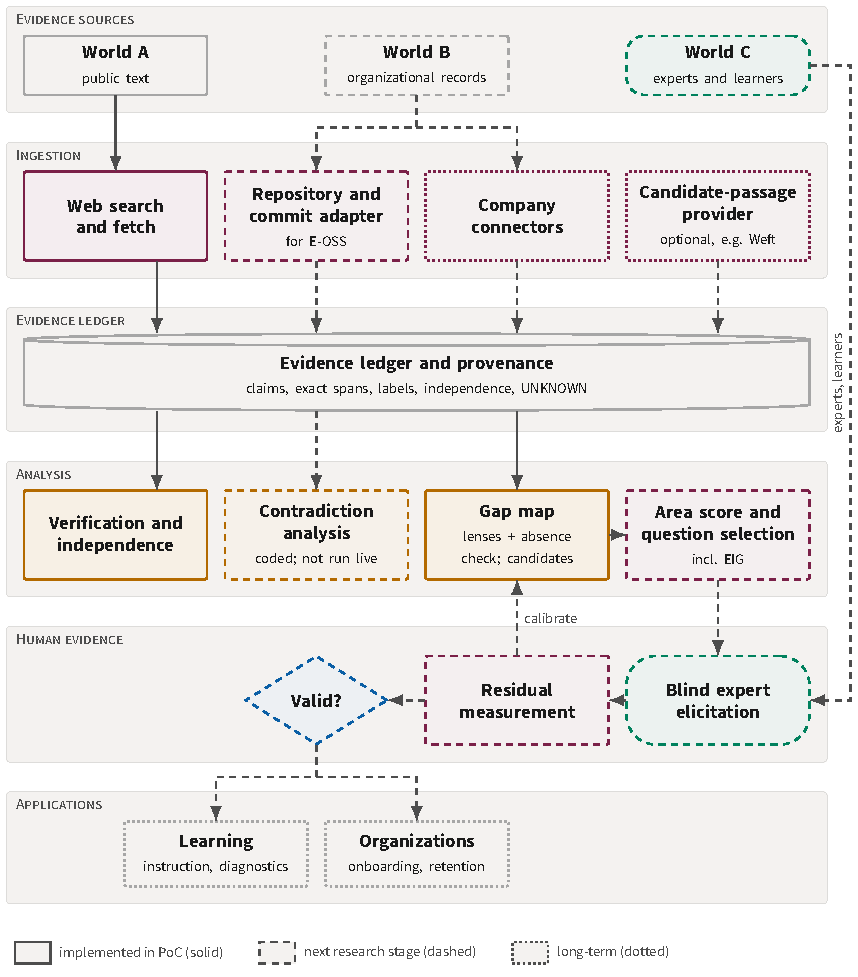
\includegraphics{figures/pdf/fig11_platform.pdf}
  \caption[Platform layers]{What would the full platform contain, and what exists today? Layers run from
    evidence sources through acquisition, provenance, the evidence ledger, analysis, the human loop and
    applications, with validation, audit and security as a rail. Solid boxes exist in the PoC; dashed
    boxes are the next research stage; dotted boxes are long-term. Only World~C evidence can score the gap
    map's predictions.}
  \label{fig:platform}
\end{figure}

\evobs{} What exists today is the evidence ledger with its frozen schema, provenance verification on open
web text, the gap map (candidates only), gates and checks, and a per-run call and cost log. Contradiction
analysis beyond the older pairwise stage, company retrieval, expert elicitation for new tracks, residual
measurement and expected-information-gain question selection are the next research stage; learner
diagnostics, instructional design and adaptive learning are long-term. \emph{Weft}, a separate public
retrieval engine, was assessed as a possible future World~B layer; it keeps no in-document character
offsets and no per-user access control, so integration is not justified now, and at most it could
supply candidate passages that the platform re-hashes and re-locates itself.

\subsection{Education}

\evlit{} Expert judgment of learner difficulty is unreliable (\cref{sec:problem}), so the education path
routes \enquote{what is difficult} through learner data alone. CTA-based instruction outperforms other
ways of identifying training content in a meta-analysis of a small number of studies ($g = 0.871$;
\cite{tofelgrehl2013cognitive}); in one biology course (N~=~314) CTA-derived instruction cut withdrawal
from 8.1\% to 1.4\% \parencite{feldon2010translating}. A worked example that prompts the learner to
generate a step beats one that states it ($g = 0.35$, $k = 6$; \cite{bisra2018selfexplanation}). But a
single item response is a poor diagnostic unit: 31\% of Force Concept Inventory answers changed on a
one-week retest \parencite{lasry2011fci}. A synthetic learner returns the misconception it was handed:
a GPT-4 simulation of that inventory showed no response variance until told which preconception to hold
\parencite{kieser2023chatgpt}. And the median effect in 747 randomized education trials was 0.10~SD
\parencite{kraft2020interpreting}.

\evint{} The pipeline is therefore evidence-complete only as far as \enquote{instructional material},
and only for items validated by humans. Synthetic learners serve only to pilot a probe or debug a
pipeline, never as evidence. A candidate education pilot would add one or two expert-confirmed operations
to self-explanation prompts in one course section and measure delayed transfer, as a feasibility pilot,
not a powered test. Validation Track~A (twelve physicists; about 370 students in a two-arm trial with
delayed transfer, futility test at $d = 0.30$) runs only on its own preconditions, with its registered
rules unchanged; this program touches it only through sealed, secondary, non-gating predictions.

\subsection{Organizations}

\evlit{} Three organizational blind spots have literature behind them: a technician's diagnostic cue,
carried in stories rather than manuals \parencite{orr1996talking}; a senior engineer's design rationale,
lost to causal ambiguity \parencite{szulanski1996exploring}; and a compliance officer's exception
judgment, the gap between work as imagined and work as done \parencite{hollnagel2018safety}. Turnover
loss is measurable in software: 65\% of 133 popular GitHub projects have a truck factor of 2 or fewer
\parencite{avelino2016novel}, and 315 of 1,932 projects (16\%) were abandoned after truck-factor
developers left \parencite{avelino2019abandonment}. \evobs{} The PoC produced candidates of the first and
third shape (the PLC GUARD record; a GDPR v2 record built on the \enquote{in most cases / in some cases}
hedge of the DPIA guidance), both unvalidated, the second from an inadmissible run.

\evhyp{} Every value proposition is untested: that a gap map shortens onboarding, turns into a capture
priority for a retiring expert, or adds predictive value beyond authorship concentration (which H-OSS
tests). We found no credible, peer-reviewed cost figure for organizational knowledge loss in general and
claim none. \evint{} The limits are hard ones. A World~B run needs access-scoped retrieval, on-premises
or contractually isolated models, re-tuned lexicons, and a data protection impact assessment; where a
German entity is involved, a works agreement. Outputs are aggregate by default, never feed performance
evaluation, and name a person only with consent. A coverage score used as a target would reward
documentation that raises the score over documentation that transfers knowledge. The recommended first
partner is a software organization, closest to the registered H-OSS design.
